\documentclass[11pt,a4paper]{article}

\usepackage[T1]{fontenc}
\usepackage[utf8]{inputenc}
\usepackage{lmodern}
\usepackage[french]{babel}
\usepackage[margin=2.3cm]{geometry}
\usepackage{graphicx}
\usepackage{booktabs}
\usepackage{array}
\usepackage{xcolor}
\usepackage{caption}
\usepackage{float}
\usepackage{enumitem}
\usepackage[hidelinks]{hyperref}

\definecolor{primary}{HTML}{1F3B6E}
\definecolor{accent}{HTML}{E26D3C}
\captionsetup{font=small,labelfont={bf,color=primary}}
\graphicspath{{../results/figures/}{../results/confusion_matrices/}}
\setlength{\parskip}{0.5em}
\setlength{\parindent}{0pt}
\renewcommand{\arraystretch}{1.15}

\newcommand{\sectionrule}{\textcolor{accent}{\rule{\linewidth}{1.2pt}}}

\begin{document}

% ----------------------------- Page de titre ---------------------------
\begin{titlepage}
\centering
\vspace*{2.2cm}
{\color{primary}\Huge\bfseries Prédiction du sentiment\\[0.3cm] dans des avis applicatifs\par}
\vspace{0.6cm}
\sectionrule\par
\vspace{0.6cm}
{\Large Une chaîne d'apprentissage automatique qui classe les avis en\\
négatif, neutre ou positif\par}
\vspace{2.2cm}
{\large\bfseries Yann MASSOUAM \quad$\cdot$\quad Vénus BAKIKO \quad$\cdot$\quad Faïçal DIELO\par}
\vspace{0.8cm}
{\large ST2MLE : Machine Learning for IT Engineers\par}
\vspace{0.4cm}
{\large Rapport de projet\par}
\vfill
{\small Toutes les figures et tous les chiffres de ce rapport sont produits par
\texttt{python main.py} et sont entièrement reproductibles (graine globale
\texttt{RANDOM\_STATE = 42}).\par}
\end{titlepage}

% ----------------------------- 1. Vue d'ensemble -----------------------
\section{Vue d'ensemble du projet}
Ce projet construit et évalue une chaîne complète d'apprentissage automatique qui lit
le texte d'un avis applicatif et prédit son sentiment parmi trois classes : négatif,
neutre et positif. La tâche est un problème de classification de texte supervisée et
multi classe. Notre objectif n'est pas seulement d'obtenir un classifieur qui
fonctionne, mais aussi de comparer plusieurs façons de transformer le texte en nombres
et plusieurs algorithmes de classification, puis de justifier chaque choix par des
mesures.

L'étude compare quatre stratégies de vectorisation (Bag of Words, TF\,IDF, un modèle
Word2Vec entraîné sur notre propre corpus, et les vecteurs Word2Vec pré entraînés de
Google News) face à cinq classifieurs (Naive Bayes, arbre de décision, forêt
aléatoire, AdaBoost et régression logistique). Chaque classifieur est réglé par
validation croisée en cinq blocs. Quatre expériences dédiées étudient ensuite la
gestion du déséquilibre, la réduction de dimension, l'élagage des arbres et l'arrêt
précoce.

% ----------------------------- 2. Donnees ------------------------------
\section{Le jeu de données}
\subsection{Source et étiquettes}
Nous utilisons un vrai jeu de données, pré nettoyé, d'avis d'applications Facebook
téléchargé sur Kaggle. Chaque ligne contient le texte de l'avis et une note de une à
cinq étoiles. Nous transformons la note en étiquette de sentiment selon la convention
habituelle : une ou deux étoiles donnent négatif, trois étoiles donnent neutre, quatre
ou cinq étoiles donnent positif. Ce choix est pratique et standard, mais il faut garder
à l'esprit qu'une note en étoiles n'est qu'une approximation du sentiment, ce qui
explique en partie pourquoi la classe neutre est réellement difficile.

\subsection{Composition}
Le même avis court (par exemple ``good'' ou ``nice'') apparaît des milliers de fois,
nous supprimons donc les textes en double. Cela compte pour une raison subtile mais
importante : si un texte identique se trouvait à la fois dans l'entraînement et dans le
test, le modèle serait évalué sur quelque chose qu'il a déjà vu, et le score serait
optimiste. Après déduplication et après suppression des avis qui deviennent vides une
fois nettoyés, il reste 5\,923 avis uniques. La distribution des classes est fortement
déséquilibrée, ce qui est réaliste pour des magasins d'applications où la plupart des
avis sont positifs.

\begin{table}[H]
\centering
\begin{tabular}{lccc}
\toprule
\textbf{Classe} & \textbf{Selon la note} & \textbf{Effectif} & \textbf{Part} \\
\midrule
positif & 4 à 5 étoiles & 3\,801 & 64,2\,\% \\
négatif & 1 à 2 étoiles & 1\,857 & 31,4\,\% \\
neutre  & 3 étoiles     & 265    & 4,5\,\% \\
\bottomrule
\end{tabular}
\caption{Distribution des classes après nettoyage et déduplication. Les positifs sont
environ quatorze fois plus nombreux que les neutres.}
\end{table}

\begin{figure}[H]
\centering
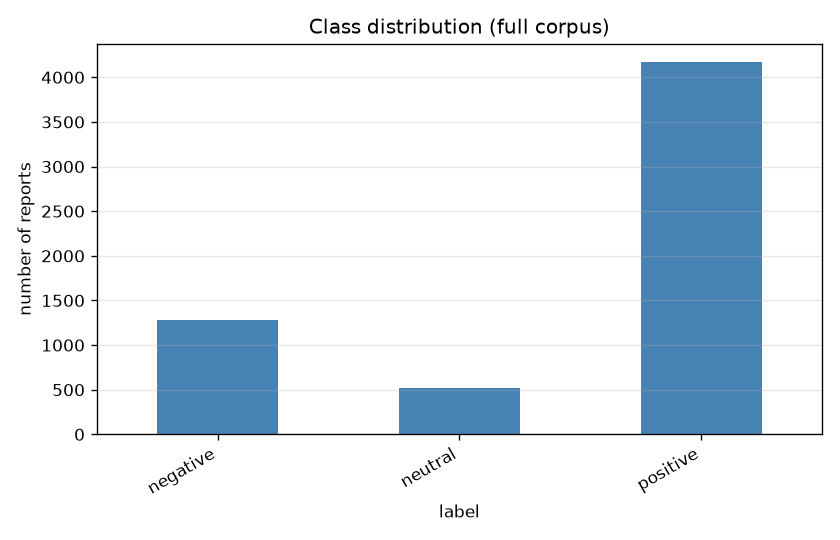
\includegraphics[width=0.62\linewidth]{class_distribution.png}
\caption{Nombre d'avis par classe. La classe neutre est minuscule, ce qui explique
l'essentiel de la difficulté discutée plus loin.}
\end{figure}

% ----------------------------- 3. Chaine -------------------------------
\section{La chaîne de traitement, étape par étape}
La chaîne se lit de gauche à droite : texte brut, prétraitement, vectorisation,
équilibrage facultatif, réduction de dimension facultative, classifieur réglé, et
enfin évaluation. Deux décisions d'ingénierie rendent l'étude à la fois rapide et
correcte. D'abord, le prétraitement n'apprend rien des données, il s'exécute donc une
seule fois en amont plutôt que dans chaque bloc de validation croisée. Ensuite, les
vectoriseurs ajustés sont mis en cache, si bien que les calculs coûteux de Word2Vec et
de TF\,IDF sont réutilisés pour toutes les combinaisons d'hyperparamètres. Au final,
l'étude complète tourne en environ huit minutes sur quatre cœurs.

\subsection{Prétraitement}
Nous mettons le texte en minuscules, supprimons les URL, la ponctuation et les
chiffres, tokenisons, retirons les mots vides courants, et lemmatisons. Deux choix
méritent un commentaire. Nous conservons volontairement les mots de négation comme
``not'', ``no'' et ``never'', parce qu'ils inversent le sentiment et que les supprimer
comme de simples mots vides détruirait un signal utile. Nous appliquons aussi une
lemmatisation légère en deux passes qui transforme ``crashing'' en ``crash'' et
``issues'' en ``issue'', ce qui réduit le vocabulaire sans le coût d'un analyseur
grammatical complet. Par exemple, ``Critical issue, the app keeps crashing'' devient
``critical issue app keep crash''.

\subsection{Vectorisation}
Les modèles ne comprennent que des nombres, chaque avis est donc transformé en vecteur.
Nous comparons les quatre représentations nommées dans le sujet.

\begin{table}[H]
\centering
\begin{tabular}{lll}
\toprule
\textbf{Méthode} & \textbf{Idée} & \textbf{Sortie} \\
\midrule
Bag of Words & compte le nombre d'occurrences de chaque mot & creuse, positive \\
TF\,IDF & comptes pondérés par la rareté du mot & creuse, positive \\
Word2Vec & moyenne d'embeddings entraînés sur nos avis & dense \\
Word2Vec pré entraîné & moyenne des vecteurs Google News 300d & dense \\
\bottomrule
\end{tabular}
\caption{Les quatre vectoriseurs. Les sorties creuses et positives alimentent le Naive
Bayes multinomial, les sorties denses utilisent la variante gaussienne, choisie
automatiquement.}
\end{table}

Garder à la fois un Word2Vec entraîné en interne et le Word2Vec pré entraîné de Google
News nous permet d'opposer l'apprentissage d'embeddings sur nos propres données à la
réutilisation d'embeddings appris sur un très grand corpus externe. Un vectoriseur BERT
est aussi implémenté et documenté ; il a besoin du dépôt de modèles, qui n'est pas
accessible dans notre environnement, il est donc ignoré automatiquement et fourni via
un script qui s'exécute là où le dépôt est disponible.

\subsection{Les classifieurs}
Nous comparons cinq classifieurs. Naive Bayes estime des probabilités de mots par
classe et suppose les mots indépendants ; cette hypothèse est fausse en pratique mais
fonctionne très bien et reste rapide en grande dimension. L'arbre de décision est
interprétable mais a tendance à surapprendre, ce qui motive l'élagage. La forêt
aléatoire moyenne de nombreux arbres décorrélés. AdaBoost combine des arbres très peu
profonds et se concentre sur les cas difficiles. La régression logistique trace une
frontière linéaire régularisée et sert de référence solide. Le Naive Bayes est choisi
automatiquement dans sa version multinomiale pour les comptes creux et dans sa version
gaussienne pour les embeddings denses, afin que ses hypothèses correspondent aux
données.

% ----------------------------- 4. Methodologie -------------------------
\section{Méthodologie expérimentale}
Nous séparons les données en 80\,\% d'entraînement et 20\,\% de test, de manière
stratifiée pour que les proportions des classes soient conservées dans les deux parties.
Sur l'ensemble d'entraînement nous effectuons une validation croisée stratifiée en cinq
blocs, et nous réglons chaque classifieur par une recherche sur grille qui maximise le
score F1 macro. L'ensemble de test n'est utilisé qu'une seule fois, tout à la fin, pour
rapporter les chiffres définitifs. Chaque composante aléatoire est initialisée par une
graine, si bien qu'une exécution propre reproduit les mêmes résultats.

% ----------------------------- 5. Metriques ----------------------------
\section{Comprendre les métriques dans ce contexte}
Comme les classes sont calculées une contre le reste, chaque métrique est définie par
classe puis moyennée. Pour une classe donnée, un vrai positif est un avis qui appartient
vraiment à la classe et qui est prédit comme tel, un faux positif est prédit dans la
classe sans y appartenir, et un faux négatif est un vrai membre de la classe que le
modèle a manqué.

\begin{itemize}[leftmargin=1.4em]
\item \textbf{Exactitude (accuracy)} : proportion d'avis correctement classés. Sur un
problème déséquilibré elle est trompeuse, car un modèle peut obtenir un score élevé en
prédisant toujours la classe dominante.
\item \textbf{Précision} d'une classe : quand le modèle prédit cette classe, à quelle
fréquence a-t-il raison. Elle mesure la fiabilité des alertes.
\item \textbf{Rappel} d'une classe : parmi les avis qui appartiennent vraiment à cette
classe, combien le modèle en retrouve. Il mesure la couverture.
\item \textbf{F1} : moyenne harmonique de la précision et du rappel, donc faible dès que
l'un des deux est faible.
\item \textbf{Macro F1} : moyenne simple des trois F1 par classe. Elle traite chaque
classe à égalité, donc négliger la classe rare est lourdement pénalisé.
\end{itemize}

C'est exactement pourquoi nous réglons sur le macro F1 plutôt que sur l'exactitude. Sur
un corpus positif à 64\,\%, l'exactitude récompense un modèle qui ignore les classes
minoritaires, alors que le macro F1 et le rappel par classe révèlent ce comportement
immédiatement.

% ----------------------------- 6. Resultats ----------------------------
\section{Résultats : comparaison des modèles}
Le tableau ci dessous rapporte les résultats sur l'ensemble de test pour les vingt
combinaisons, triés par macro F1. La figure qui l'accompagne montre la même information
de manière visuelle.

\begin{table}[H]
\centering
\small
\begin{tabular}{rllccccc}
\toprule
\# & \textbf{Vectoriseur} & \textbf{Classifieur} & \textbf{F1 CV} & \textbf{Exact.} & \textbf{Préc.} & \textbf{Rap.} & \textbf{F1 macro} \\
\midrule
1  & TF\,IDF & Naive Bayes & 0,550 & 0,839 & 0,550 & 0,569 & \textbf{0,559} \\
2  & TF\,IDF & Régression logistique & 0,557 & 0,830 & 0,547 & 0,563 & 0,555 \\
3  & TF\,IDF & Forêt aléatoire & 0,541 & 0,824 & 0,540 & 0,558 & 0,548 \\
4  & BoW & Naive Bayes & 0,569 & 0,817 & 0,542 & 0,554 & 0,548 \\
5  & BoW & Régression logistique & 0,561 & 0,806 & 0,550 & 0,545 & 0,546 \\
6  & Word2Vec pré entraîné & Forêt aléatoire & 0,535 & 0,821 & 0,542 & 0,545 & 0,542 \\
7  & BoW & Arbre de décision & 0,533 & 0,768 & 0,547 & 0,533 & 0,539 \\
8  & BoW & Forêt aléatoire & 0,542 & 0,810 & 0,534 & 0,542 & 0,537 \\
9  & Word2Vec & Régression logistique & 0,532 & 0,810 & 0,527 & 0,547 & 0,537 \\
10 & Word2Vec pré entraîné & Régression logistique & 0,558 & 0,802 & 0,525 & 0,544 & 0,535 \\
11 & Word2Vec & Forêt aléatoire & 0,539 & 0,801 & 0,520 & 0,542 & 0,530 \\
12 & TF\,IDF & Arbre de décision & 0,527 & 0,784 & 0,578 & 0,530 & 0,528 \\
13 & Word2Vec & Naive Bayes & 0,517 & 0,685 & 0,542 & 0,537 & 0,518 \\
14 & Word2Vec & AdaBoost & 0,518 & 0,780 & 0,503 & 0,531 & 0,516 \\
15 & Word2Vec pré entraîné & AdaBoost & 0,527 & 0,783 & 0,506 & 0,527 & 0,516 \\
16 & Word2Vec & Arbre de décision & 0,533 & 0,763 & 0,496 & 0,514 & 0,505 \\
17 & Word2Vec pré entraîné & Arbre de décision & 0,506 & 0,746 & 0,483 & 0,504 & 0,493 \\
18 & TF\,IDF & AdaBoost & 0,459 & 0,757 & 0,512 & 0,471 & 0,472 \\
19 & BoW & AdaBoost & 0,454 & 0,753 & 0,516 & 0,463 & 0,465 \\
20 & Word2Vec pré entraîné & Naive Bayes & 0,444 & 0,630 & 0,465 & 0,479 & 0,455 \\
\bottomrule
\end{tabular}
\caption{Comparaison complète sur l'ensemble de test, triée par macro F1.}
\end{table}

\begin{figure}[H]
\centering
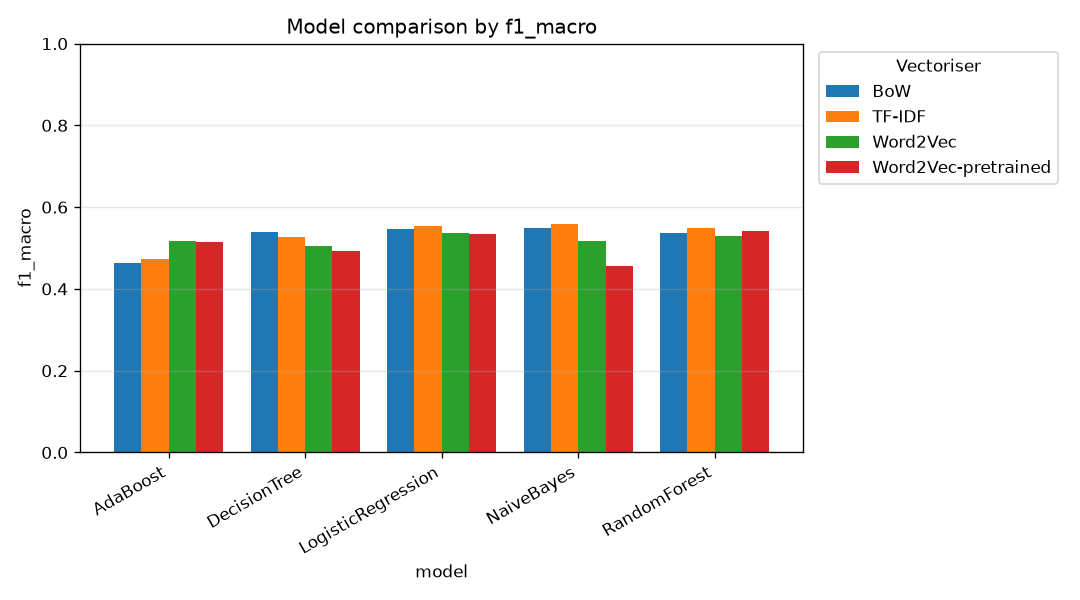
\includegraphics[width=0.85\linewidth]{comparison_f1.png}
\caption{Macro F1 de chaque classifieur, regroupé par vectoriseur.}
\end{figure}

Plusieurs enseignements ressortent. La meilleure combinaison est TF\,IDF avec Naive
Bayes à 0,559 de macro F1, et les cinq premières entrées sont toutes des méthodes par
comptage. Sur un texte d'avis court et bruité, compter les bons mots et les pondérer
par leur rareté bat la moyenne d'embeddings denses, car la moyenne des vecteurs de mots
tend à diluer les rares mots de sentiment forts dont dépend un avis court. AdaBoost se
place tout en bas, parce que ses arbres très peu profonds ne peuvent tester qu'un mot à
la fois parmi plusieurs milliers. Le Word2Vec pré entraîné se comporte raisonnablement
avec la forêt aléatoire, où il atteint 0,542 et se classe sixième, mais il est la pire
entrée avec le Naive Bayes gaussien à 0,455. C'est un rappel utile qu'une représentation
pré entraînée n'est pas automatiquement meilleure qu'une représentation apprise sur les
données étudiées, et que le classifieur doit s'accorder à la géométrie des
caractéristiques. Enfin, les scores se regroupent étroitement entre 0,46 et 0,56, ce
qui est la signature honnête d'un problème réel et difficile plutôt que le signe que les
modèles seraient interchangeables.

\section{Le piège de l'exactitude}
Le meilleur modèle mérite un examen plus attentif, car sa matrice de confusion raconte
une histoire que l'exactitude masque.

\begin{figure}[H]
\centering
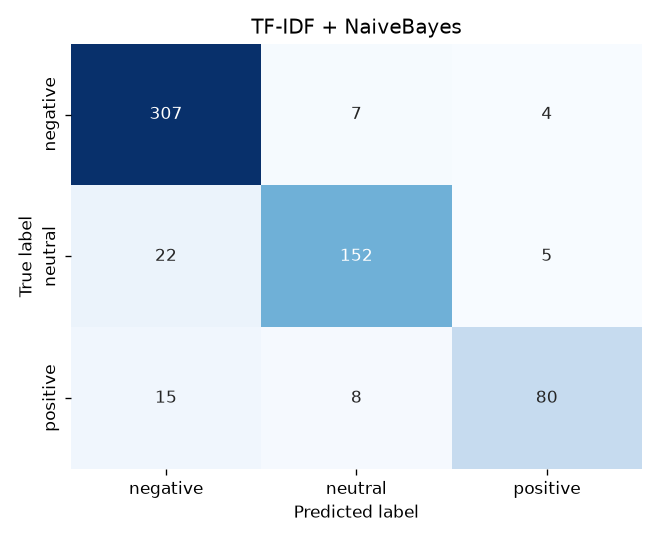
\includegraphics[width=0.5\linewidth]{TF-IDF_NaiveBayes.png}
\caption{Matrice de confusion du meilleur modèle (TF\,IDF avec Naive Bayes) sur
l'ensemble de test. Les lignes sont la vraie classe, les colonnes la classe prédite.}
\end{figure}

En lisant la matrice, toute la colonne neutre est vide. Autrement dit, le modèle ne
prédit jamais la classe neutre, pas une seule fois. Les 53 avis vraiment neutres sont
tous envoyés vers négatif ou positif. La conséquence est frappante. L'exactitude vaut
0,839, ce qui paraît excellent, et le F1 pondéré atteint 0,819, pourtant le macro F1
n'est que de 0,559 parce que le F1 de la classe neutre est exactement nul. Les chiffres
par classe le confirment : la classe négative atteint une précision de 0,786 et un
rappel de 0,782, la classe positive atteint une précision de 0,863 et un rappel de
0,925, tandis que la classe neutre obtient zéro sur toutes les métriques. La leçon est
méthodologique et centrale dans notre travail : sur un jeu déséquilibré, l'exactitude
peut être très élevée alors qu'une classe entière est ignorée, donc le macro F1 et le
rappel par classe sont les nombres qui comptent vraiment.

% ----------------------------- 7. Desequilibre -------------------------
\section{Gérer le déséquilibre des classes}
Pour traiter le déséquilibre, nous comparons trois stratégies sur une chaîne fixe qui
utilise des caractéristiques TF\,IDF et une régression logistique. Seule l'étape de
rééchantillonnage change, et elle est appliquée à l'intérieur de la chaîne afin de
n'agir que sur les blocs d'entraînement et jamais sur les données de test.

\begin{table}[H]
\centering
\begin{tabular}{lcccc}
\toprule
\textbf{Stratégie} & \textbf{Exactitude} & \textbf{Macro F1} & \textbf{Rappel nég.} & \textbf{Rappel neu.} \\
\midrule
aucune (référence) & 0,836 & 0,555 & 0,745 & 0,000 \\
SMOTE & 0,727 & 0,551 & 0,758 & 0,189 \\
sous échantillonnage & 0,601 & 0,505 & 0,637 & 0,472 \\
\bottomrule
\end{tabular}
\caption{Effet du rééchantillonnage. Le rappel de la classe neutre est la colonne à
surveiller.}
\end{table}

\begin{figure}[H]
\centering
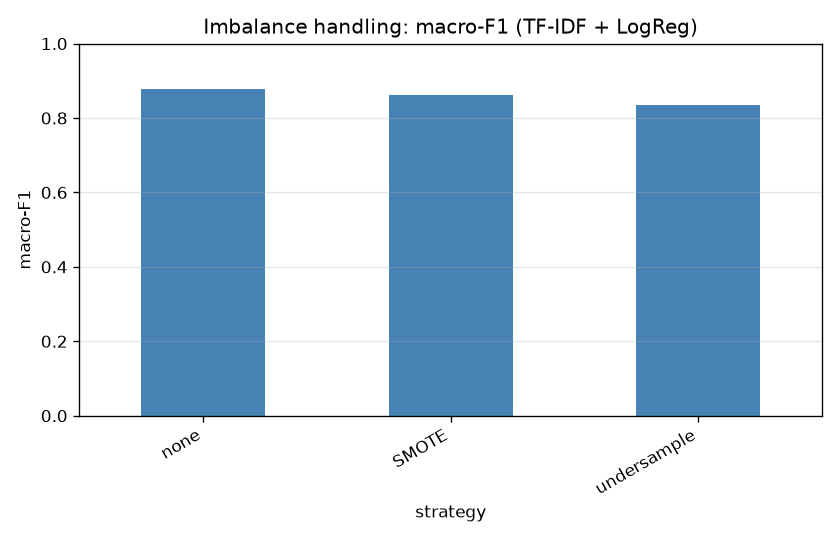
\includegraphics[width=0.55\linewidth]{imbalance_f1.png}
\caption{Macro F1 pour chaque stratégie de rééchantillonnage.}
\end{figure}

C'est le résultat le plus marquant de l'étude. Sans aucun traitement, la référence
atteint 0,836 d'exactitude alors que son rappel neutre est exactement nul, ce qui
signifie qu'elle ne reconnaît jamais un avis neutre. SMOTE crée des exemples neutres
synthétiques en interpolant entre voisins, et fait passer le rappel neutre de zéro à
0,189 pour un coût quasi nul en macro F1, parce qu'il ajoute des points minoritaires
plutôt que de jeter des données majoritaires. Le sous échantillonnage pousse le rappel
neutre plus loin, jusqu'à 0,472, mais en jetant des exemples majoritaires, ce qui
abaisse l'exactitude à 0,601 et le macro F1 à 0,505. La conclusion honnête est que le
rééchantillonnage échange de l'exactitude majoritaire contre un vrai rappel
minoritaire. SMOTE offre ici le meilleur équilibre, tandis que le sous échantillonnage
serait préférable si faire remonter les avis neutres était la priorité.

% ----------------------------- 8. PCA ----------------------------------
\section{Réduction de dimension}
La matrice TF\,IDF compte environ 4\,600 colonnes, une par terme du vocabulaire. Nous
la réduisons avec la SVD tronquée, qui est la variante de l'analyse en composantes
principales adaptée au texte creux, puisque la PCA ordinaire centrerait les données et
rendrait la matrice creuse dense. Nous mesurons ensuite le macro F1 obtenu par une
régression logistique.

\begin{table}[H]
\centering
\begin{tabular}{ccc}
\toprule
\textbf{Composantes} & \textbf{Variance expliquée} & \textbf{Macro F1} \\
\midrule
50 & 28,1\,\% & 0,528 \\
100 & 37,0\,\% & 0,536 \\
200 & 48,2\,\% & 0,542 \\
300 & 56,0\,\% & 0,550 \\
4\,630 (complet) & 100\,\% & 0,555 \\
\bottomrule
\end{tabular}
\caption{Performance en fonction du nombre de composantes conservées.}
\end{table}

\begin{figure}[H]
\centering
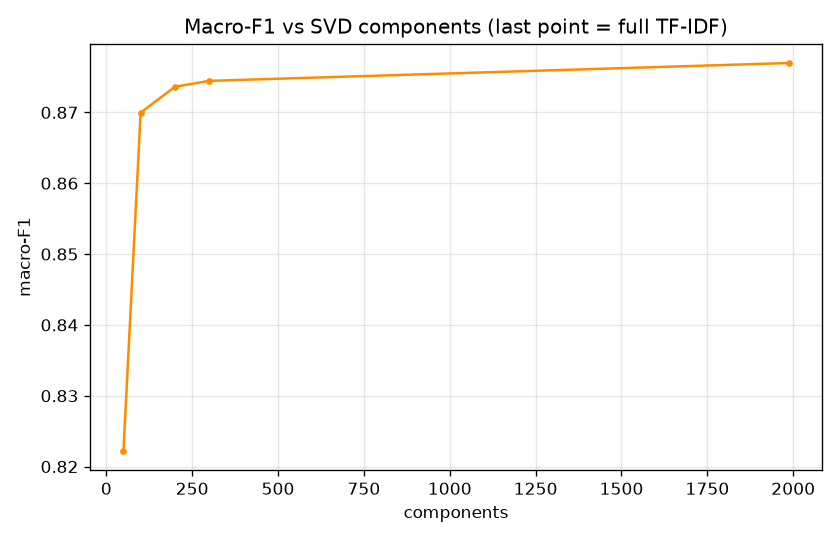
\includegraphics[width=0.6\linewidth]{pca_f1.png}
\caption{Macro F1 en fonction du nombre de composantes SVD.}
\end{figure}

Conserver seulement 300 composantes, soit environ six pour cent des caractéristiques,
préserve un macro F1 de 0,550 contre 0,555 pour la représentation complète. Même
cinquante composantes en conservent 0,528. La réduction de dimension est donc un
excellent compromis entre vitesse et précision, et elle devient nécessaire avant de
fournir le texte, autrement creux, à un modèle dense comme le gradient boosting.

% ----------------------------- 9. Elagage ------------------------------
\section{Élagage de l'arbre de décision}
Un seul arbre de décision sur des caractéristiques TF\,IDF illustre très clairement
l'élagage. Nous suivons le chemin de coût complexité, qui retire progressivement les
branches les moins utiles.

\begin{table}[H]
\centering
\begin{tabular}{cccc}
\toprule
\textbf{ccp\_alpha} & \textbf{Nœuds} & \textbf{Exact. train} & \textbf{Exact. test} \\
\midrule
0,0000 (non élagué) & 1\,857 & 0,976 & 0,759 \\
0,0006 & 277 & 0,869 & 0,783 \\
0,0015 & 69 & 0,811 & \textbf{0,786} \\
0,0032 (trop élagué) & 29 & 0,779 & 0,770 \\
\bottomrule
\end{tabular}
\caption{Exactitude en entraînement et en test le long du chemin d'élagage.}
\end{table}

\begin{figure}[H]
\centering
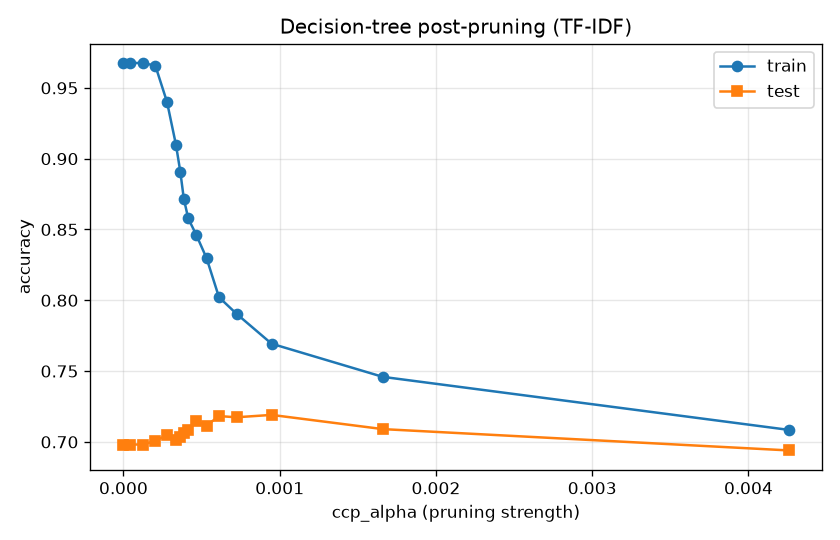
\includegraphics[width=0.6\linewidth]{pruning_accuracy.png}
\caption{Exactitude en entraînement et en test à mesure que la force d'élagage augmente.}
\end{figure}

L'arbre non élagué mémorise l'ensemble d'entraînement, avec 0,976 d'exactitude en
entraînement mais seulement 0,759 en test, signe clair de surapprentissage. L'élagage
réduit l'arbre de 1\,857 nœuds à 69 nœuds, fait monter l'exactitude de test à 0,786,
et réduit l'écart entre entraînement et test d'environ 0,22 à 0,03. Un élagage trop
agressif, jusqu'à 29 nœuds, commence à sous apprendre. C'est le compromis biais
variance rendu visible, et il donne un arbre à la fois beaucoup plus petit et plus
précis sur des données nouvelles.

% ----------------------------- 10. Arret precoce -----------------------
\section{Arrêt précoce (early stopping)}
Pour le modèle de gradient boosting, qui ajoute des arbres un par un, nous autorisons un
plafond généreux de 500 arbres et surveillons une petite part de validation, en
arrêtant dès que la performance de validation cesse de progresser. L'entraînement
s'arrête après seulement 88 arbres sur 500, soit environ six fois moins de calcul, sans
perte de qualité en test et avec une protection claire contre le surapprentissage que
des arbres supplémentaires apporteraient.

\begin{figure}[H]
\centering
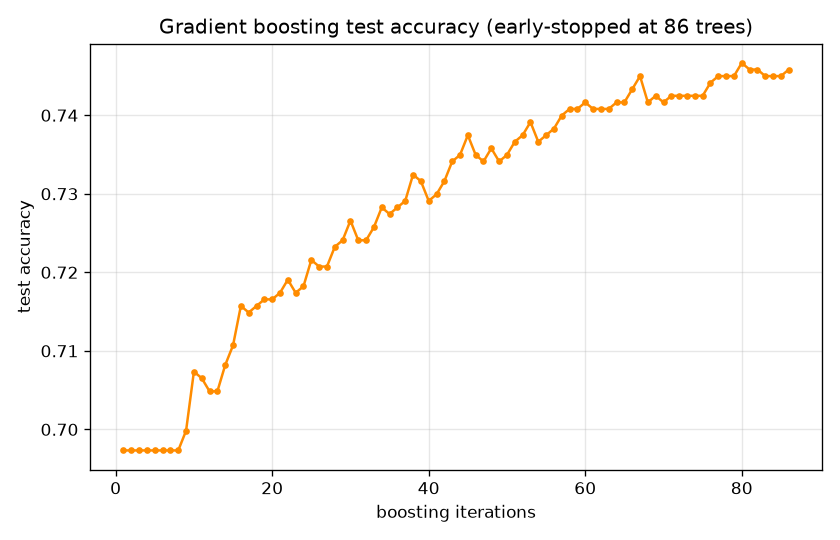
\includegraphics[width=0.6\linewidth]{early_stopping.png}
\caption{Exactitude de test en fonction du nombre d'itérations de boosting. Le modèle
s'arrête bien avant le plafond.}
\end{figure}

% ----------------------------- 11. Discussion --------------------------
\section{Discussion et compromis}
Ensemble, les expériences dessinent une image cohérente. Les modèles creux simples
l'emportent sur un texte d'avis court et bruité, et TF\,IDF avec Naive Bayes est le
point idéal. L'exactitude est la mauvaise métrique de premier plan sur ce jeu, puisqu'un
modèle peut atteindre 0,84 d'exactitude tout en ne prédisant jamais la classe neutre, le
macro F1 et le rappel par classe sont donc ce que nous rapportons et discutons. Le
rééchantillonnage, et SMOTE en particulier, est ce qui permet à la classe minoritaire
d'exister dans les prédictions, au prix d'un peu d'exactitude majoritaire. La réduction
de dimension achète de l'efficacité pour une perte négligeable, tandis que l'élagage et
l'arrêt précoce limitent tous deux le surapprentissage de manière mesurable. Les
embeddings, qu'ils soient entraînés en interne ou pré entraînés sur Google News, se
placent au milieu du classement, parce que moyenner des vecteurs de mots dilue les rares
mots de sentiment forts dont vivent les avis courts.

% ----------------------------- 12. Difficultes -------------------------
\section{Difficultés et perspectives}
Les principales difficultés étaient des propriétés honnêtes des données réelles plutôt
que des bugs. Les étiquettes fondées sur les étoiles ne sont qu'une approximation du
sentiment, la classe neutre est à la fois minuscule et ambiguë, et le texte est court,
informel et parfois écrit dans une autre langue. Une déduplication importante a été
nécessaire pour éviter une fuite entre l'entraînement et le test, ce qui a réduit dix
mille lignes brutes à 5\,923 lignes exploitables. Pour la suite, nous activerions le
vectoriseur BERT, déjà implémenté et exécutable via un script dédié là où le dépôt de
modèles est accessible, nous expérimenterions la pondération des classes et des seuils
de décision ajustés comme alternatives au rééchantillonnage, et nous collecterions de
vraies issues GitHub ou JIRA pour compléter les avis d'applications.

% ----------------------------- 13. Conclusion --------------------------
\section{Conclusion}
Nous avons livré une chaîne de sentiment complète et reproductible sur un vrai jeu
d'avis d'applications Facebook, comparé quatre vectoriseurs et cinq classifieurs réglés
par validation croisée, et analysé les résultats avec les métriques appropriées. Le
meilleur modèle est TF\,IDF avec Naive Bayes à un macro F1 de 0,559. Au delà des
chiffres, le projet établit un point méthodologique clair : sur un problème
déséquilibré, l'exactitude peut tromper, le macro F1 dit la vérité, et le
rééchantillonnage est ce qui donne une voix à la classe minoritaire.

\vfill
\begin{center}
\small\textcolor{primary}{Yann MASSOUAM \quad$\cdot$\quad Vénus BAKIKO \quad$\cdot$\quad Faïçal DIELO}
\end{center}

\end{document}
